\subsection{Class Diagram}


The main structure of the class diagram is divided into two parts: one for the filter package and the other for the Servlet package. The filter package, shown at the bottom left of the diagram, is relatively easy to read. The LoginFilter class extends the AbstractFilter class. For the rest of the classes, there are twelve resources to handle, from analytics to users. Among these resources, Activities, Template, and Analytics use a single servlet to implement CRUD queries, while others employ the REST paradigm. Specifically, we can compare and contrast the TemplateServlet and UserRestResource to understand the entire class diagram.\\

Regarding users, multiple servlets are used to handle the user resource. In particular, there is a servlet (UserServlet) that is mapped to URIs that are freely accessible from outside.\\

In the case of the Template resource, it uses a servlet (TemplateServlet) to handle it. The TemplateServlet utilizes the DoGet, DoPost, and DoDelete methods provided by the HttpServlet class to get, delete, update, and insert templates. TemplateServlet also has several subclasses. For instance, it overrides the "DeletionOperations" method to delete the template by the template ID. In this subclass, it calls the Data Access Objects (DAOs) DeleteTemplateDatabase to access data in the database. Note that TemplateServlet is mainly kept for legacy reasons.\\

Regarding the User resource, the servlet that implements the required behaviors to handle it is a more traditional servlet based on the REST paradigm. In particular, there is a servlet that handles the Users resource and parses the URI to determine the type (and possibly the ID) of the resource that the user wants to interact with. Once the servlet has processed the request, it forwards it to the proper Rest Manager class. There are six Rest Manager classes, including UserRestResource, which is a subclass of RestResource and implements the methods to handle the proper resource.\\
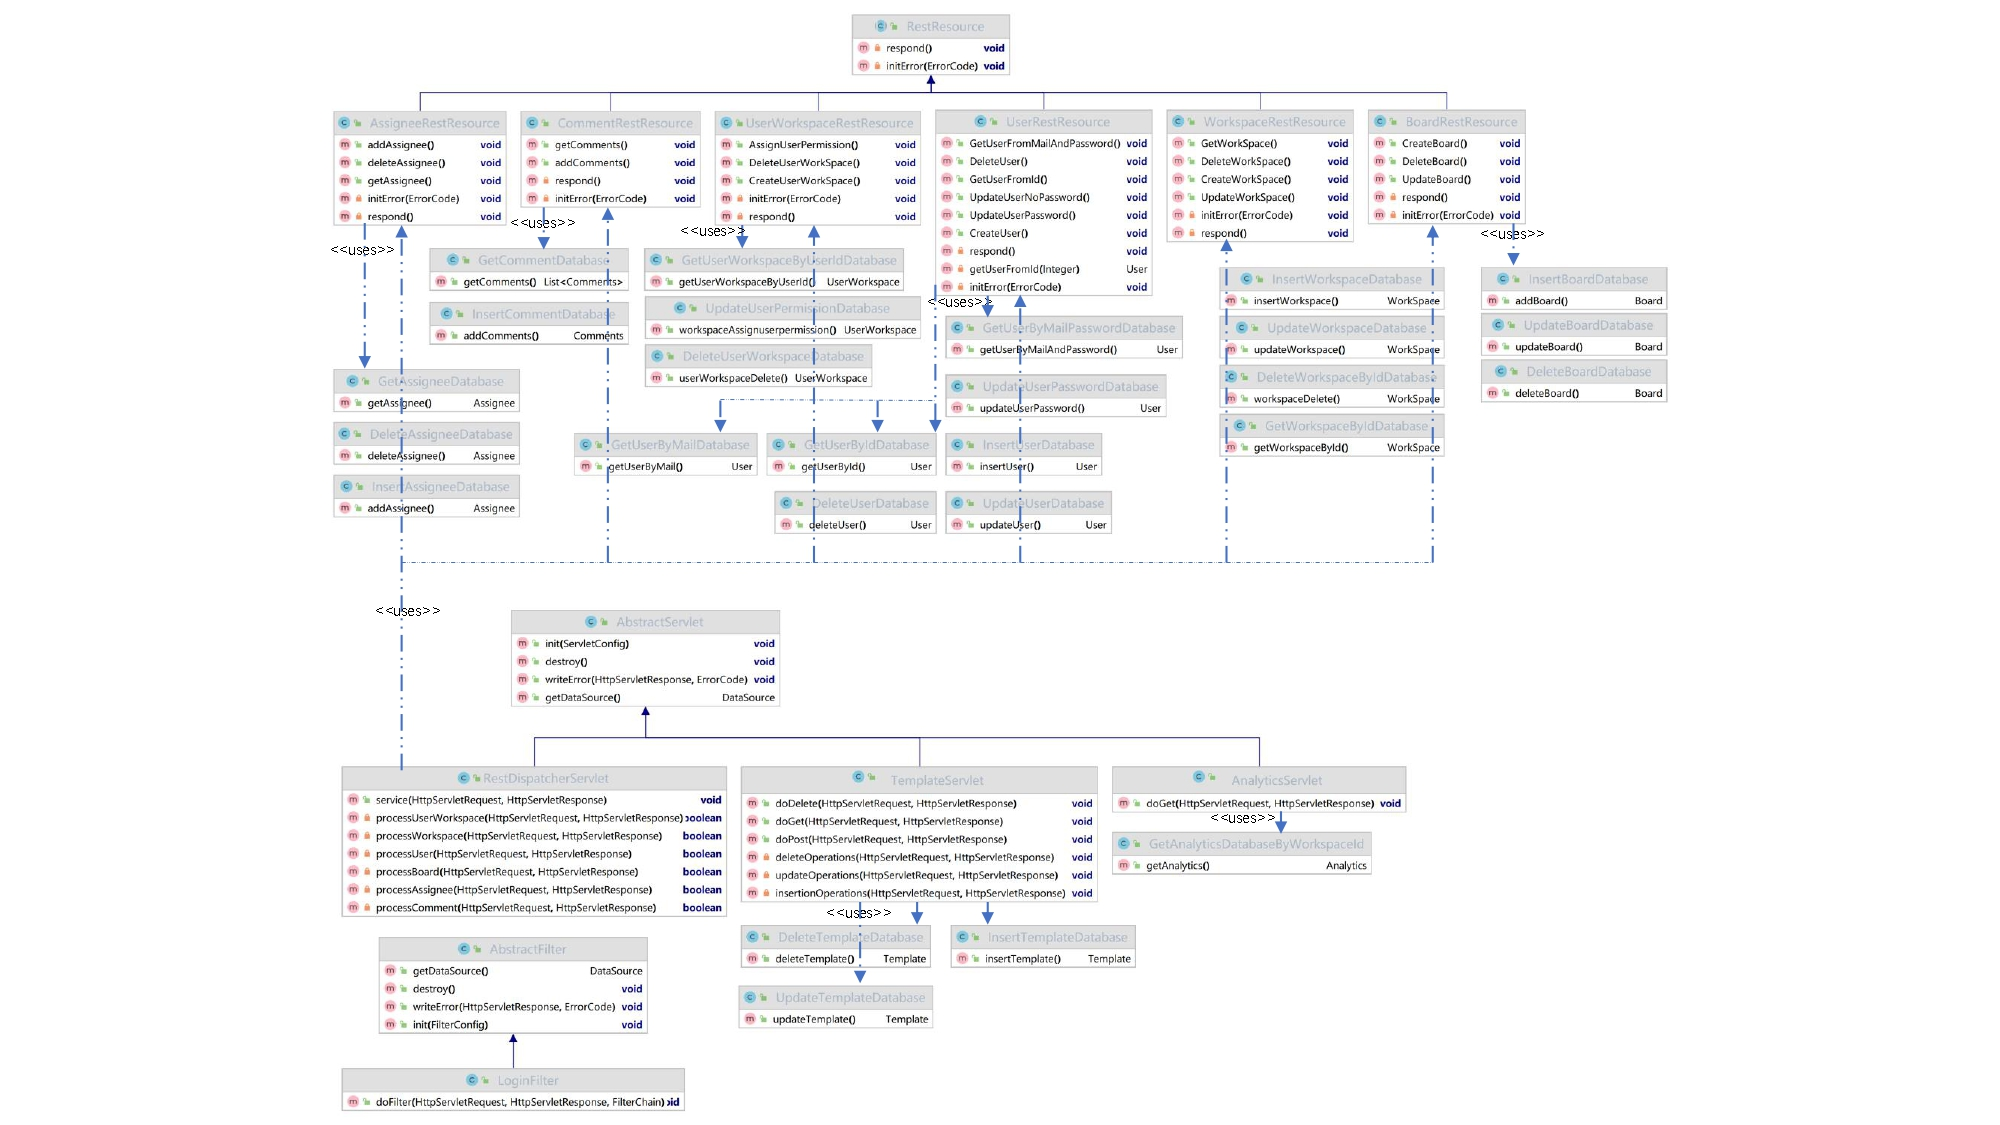
\includegraphics[width=1.30\columnwidth]{images/class sequence.jpg}\\

\subsection{Sequence Diagram}
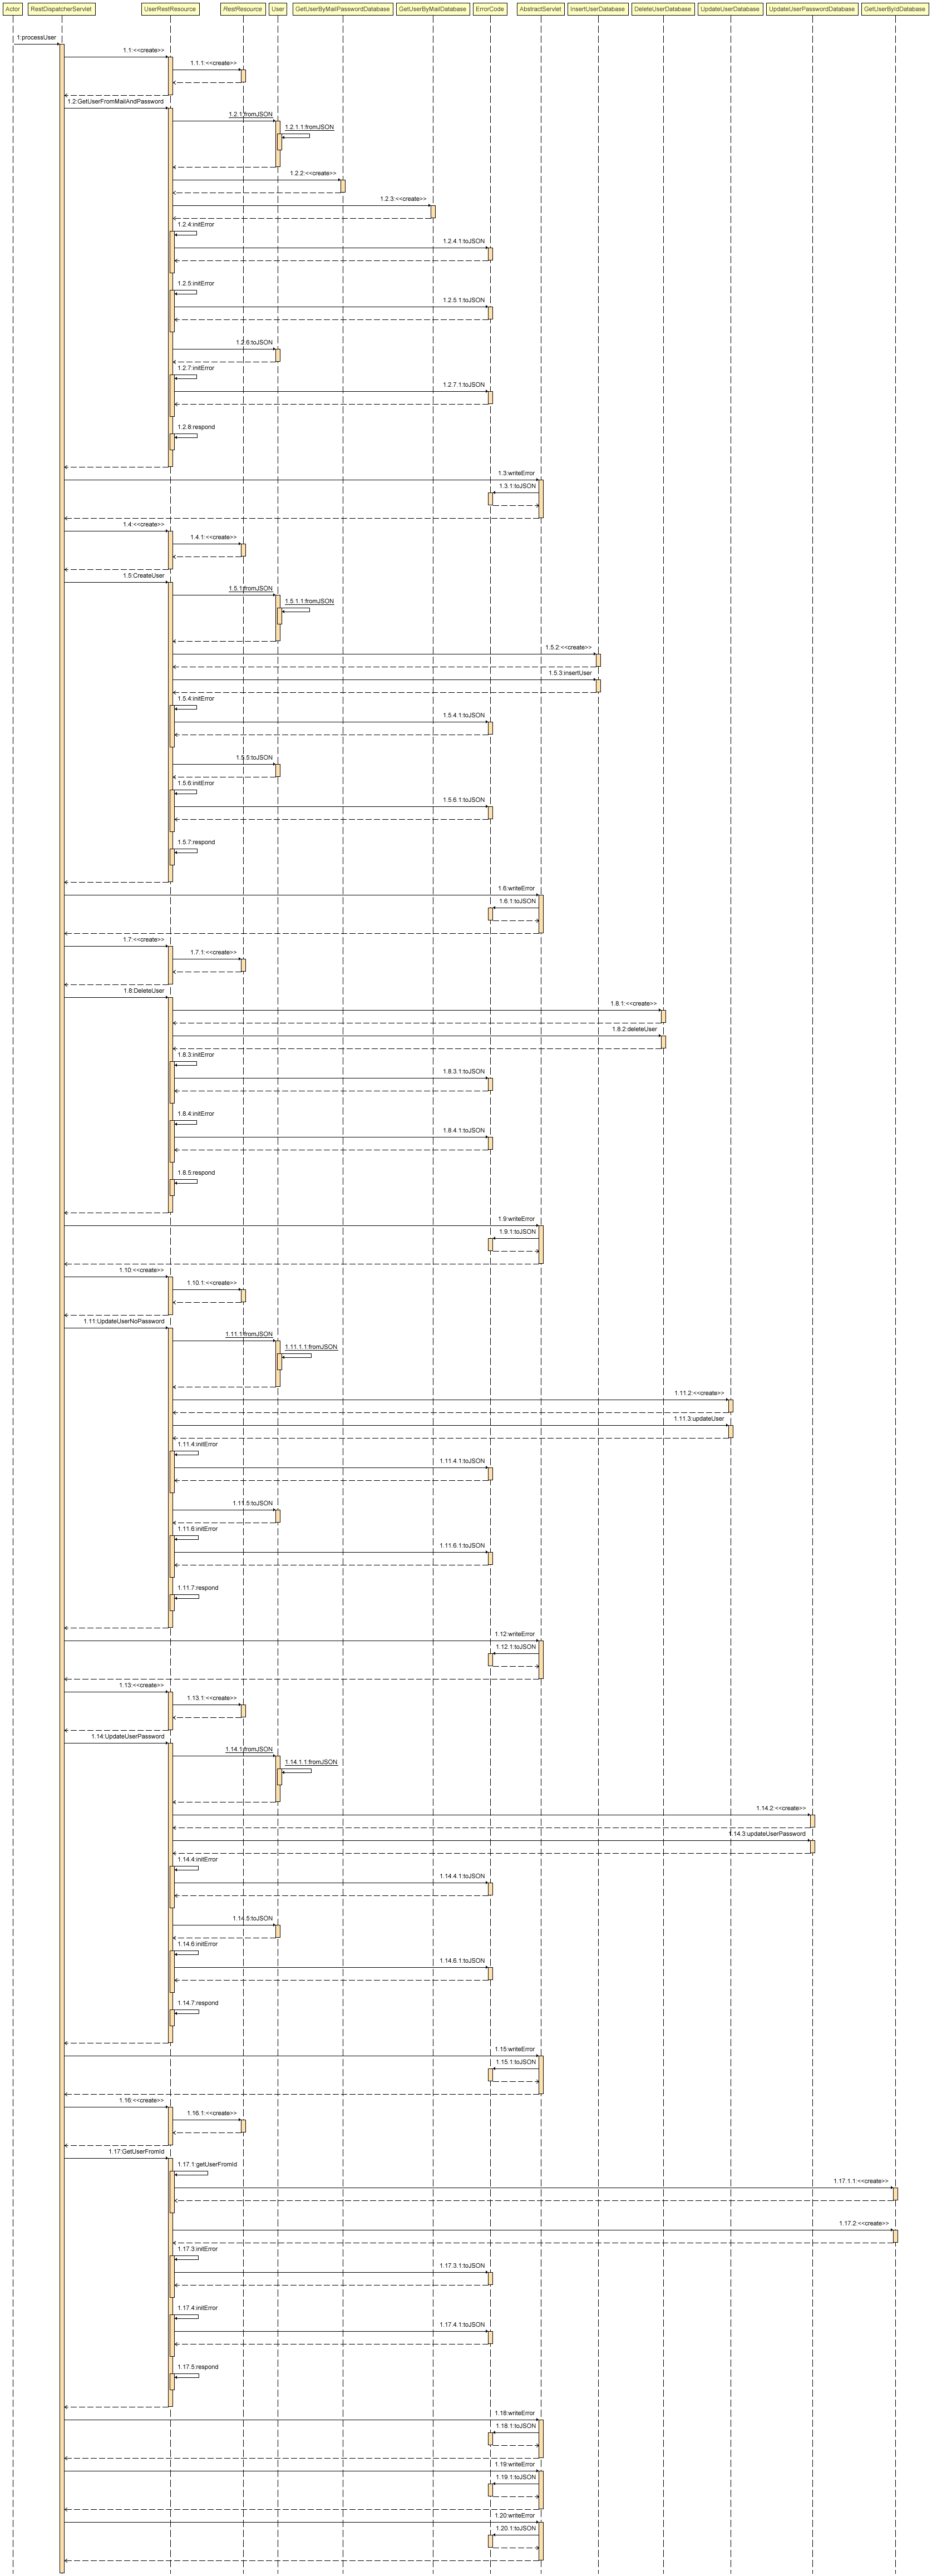
\includegraphics[width=0.5\columnwidth]{images/RestDispatcherServlet_processUser.jpg}